\chapter{Material complementario del caso real}
\label{app:caso_real_complementario}

Este anexo recoge material de apoyo del caso real de \textit{Hermetia illucens}. El objetivo es documentar la trazabilidad del dataset modelado y aportar figuras complementarias que ayudan a interpretar los resultados del Capítulo~\ref{chap:diseno_experimental}, sin sustituir las figuras principales de generalización LODO, comparación de kernels, incertidumbre y pre-\emph{infill}.

\section{Inventario de datasets generados}
\label{app:inventario_datasets_entomotive}

El flujo de preparación genera varios datasets a partir de los archivos experimentales originales. Sin embargo, el modelado del caso real se limita al dataset de productividad de \textit{Hermetia}, por las razones de alcance y homogeneidad descritas en el Capítulo~\ref{chap:diseno_experimental}. El Cuadro~\ref{tab:app_inventory_entomotive} resume los datasets generados y su papel en el trabajo.

\begin{table}[htbp]
\centering
\small
\caption[Inventario de datasets Entomotive]{Inventario de datasets generados en el caso Entomotive.}
\label{tab:app_inventory_entomotive}
\renewcommand{\arraystretch}{1.15}
\begin{tabularx}{\textwidth}{@{}p{5.3cm} p{1.4cm} p{1.7cm} p{2cm} X@{}}
\toprule
\textbf{Dataset} & \textbf{Filas} & \textbf{Dietas} & \textbf{Especie} & \textbf{Uso} \\
\midrule
\texttt{productivity\_hermetia\_lote.csv} & 33 & 11 & \textit{Hermetia} & Dataset modelado en el flujo de preparación del caso real. \\
\texttt{productivity\_tenebrio\_lote.csv} & 57 & 19 & \textit{Tenebrio} & Dataset generado disponible, no modelado en los resultados actuales. \\
\texttt{productivity\_all\_lote.csv} & 90 & 19 & Ambas & Dataset combinado disponible para análisis posteriores. \\
\texttt{quality\_hermetia\_dieta.csv} & 11 & 11 & \textit{Hermetia} & Dataset de calidad de dieta generado como soporte. \\
\texttt{quality\_tenebrio\_dieta.csv} & 19 & 19 & \textit{Tenebrio} & Dataset de calidad de dieta generado como soporte. \\
\texttt{quality\_all\_dieta.csv} & 30 & 19 & Ambas & Dataset combinado de calidad disponible. \\
\bottomrule
\end{tabularx}
\end{table}
\FloatBarrier

En el dataset modelado, las 33 observaciones corresponden a 11 dietas con tres réplicas por dieta. Los objetivos utilizados son \texttt{FCR}, \texttt{QUITINA (\%)} y \texttt{PROTEINA (\%)}. La disponibilidad es completa para quitina y proteína, con 33 valores válidos, y ligeramente menor para FCR, con 31 valores válidos.

\section{Valores observados por dieta}
\label{app:valores_observados_dieta}

La Figura~\ref{fig:app_real_dataset_targets_by_diet} resume los valores medios observados por dieta para los tres objetivos del caso real. Esta figura no se utiliza como resultado principal del modelo, sino como comprobación descriptiva previa: permite ver que los mejores valores observados no pertenecen siempre a la misma dieta y que el problema tiene una naturaleza multiobjetivo.

\begin{figure}[htbp]
\centering
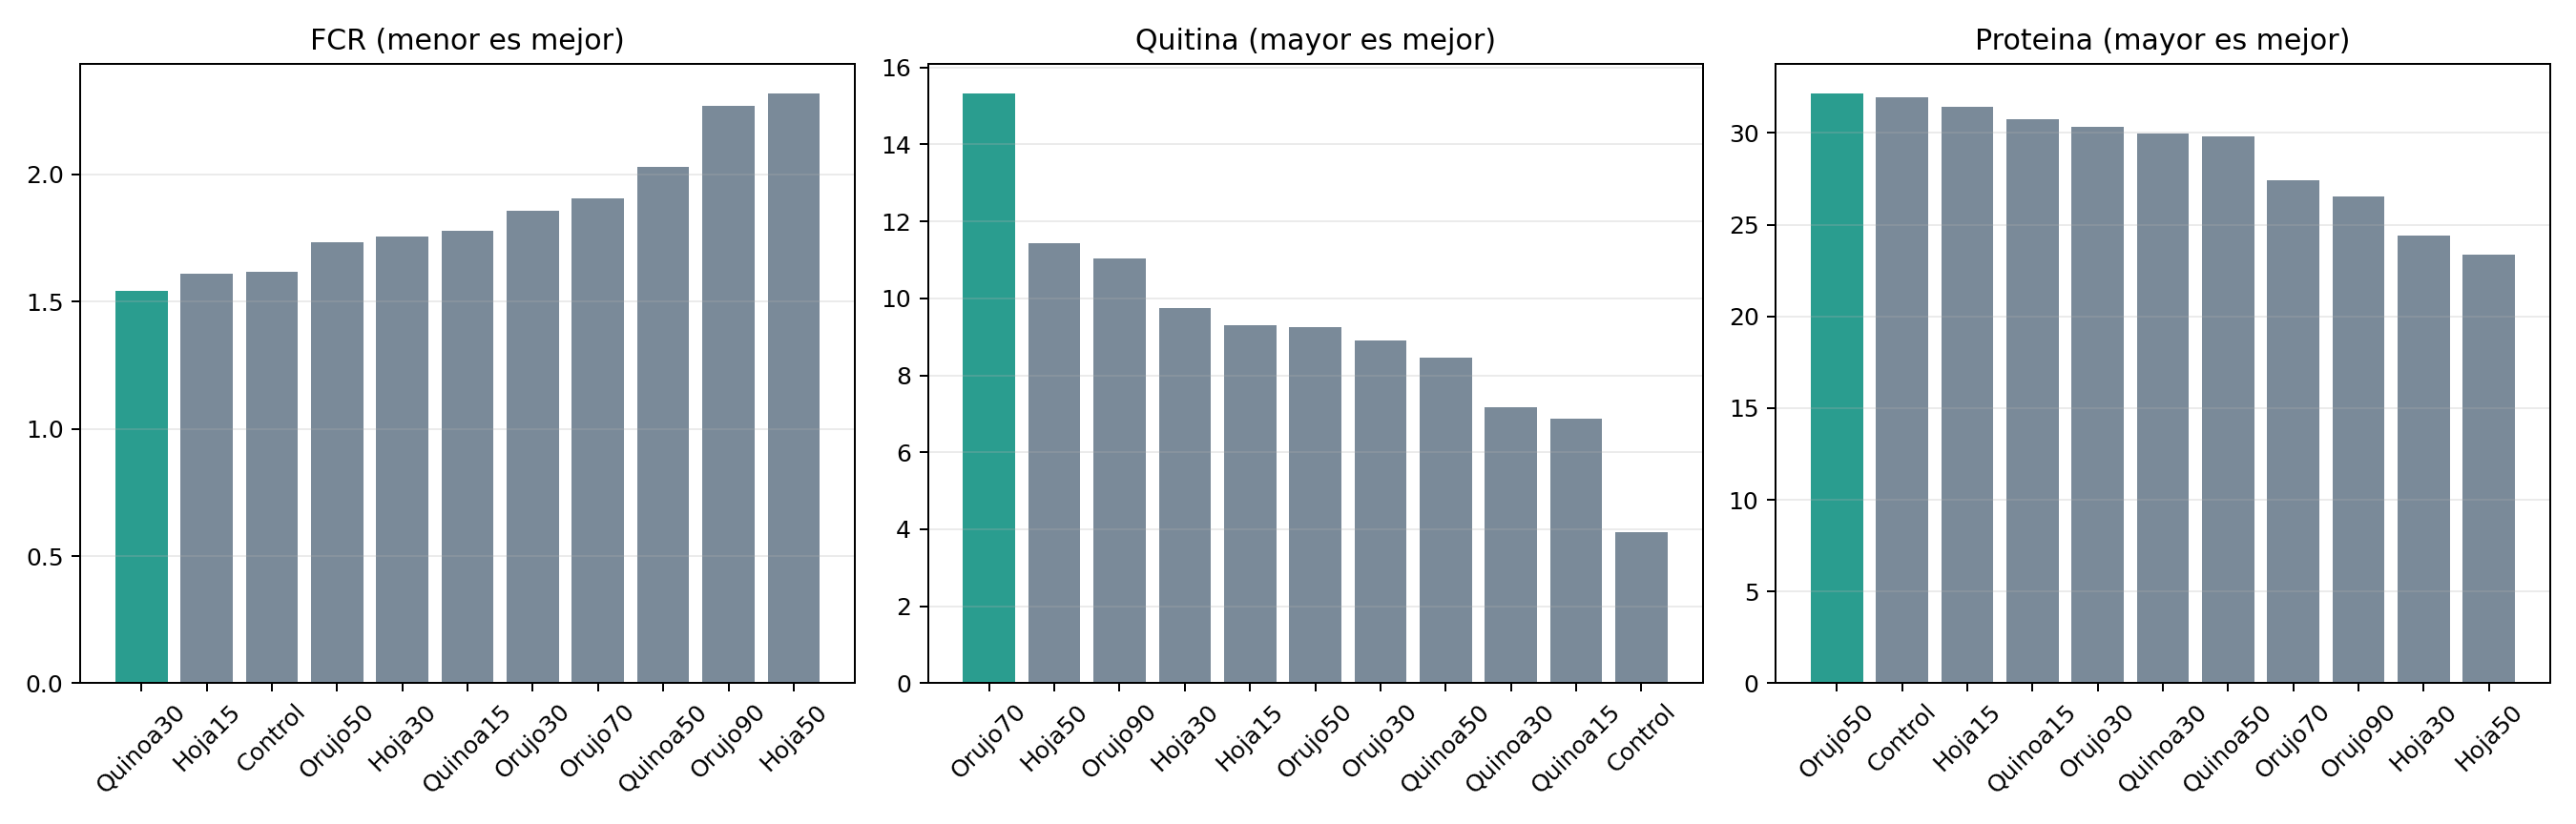
\includegraphics[width=\textwidth]{assets/app_real_dataset_targets_by_diet.png}
\caption[Valores observados por dieta]{Valores medios observados por dieta para FCR, quitina y proteína en el dataset de \textit{Hermetia}. En FCR valores menores son mejores; en quitina y proteína valores mayores son mejores.}
\label{fig:app_real_dataset_targets_by_diet}
\end{figure}
\FloatBarrier

\begin{table}[htbp]
\centering
\small
\caption[Mejores dietas observadas por objetivo]{Mejores dietas observadas por objetivo individual.}
\label{tab:app_observed_incumbents_real_case}
\renewcommand{\arraystretch}{1.15}
\begin{tabularx}{\textwidth}{@{}p{3.0cm} p{2.2cm} p{2.4cm} p{2.6cm} X@{}}
\toprule
\textbf{Objetivo} & \textbf{Criterio} & \textbf{Dieta} & \textbf{Subproducto} & \textbf{Valor medio observado} \\
\midrule
FCR & Minimizar & Quinoa30 & quinoa & 1.543 \\
Quitina & Maximizar & Orujo70 & orujo & 15.318 \\
Proteína & Maximizar & Orujo50 & orujo & 32.147 \\
\bottomrule
\end{tabularx}
\end{table}
\FloatBarrier

\section{Paridad del mejor GP por objetivo}
\label{app:paridad_mejor_gp_real_case}

La Figura~\ref{fig:app_real_best_gp_parity_by_target} complementa las métricas agregadas del Capítulo~\ref{chap:diseno_experimental}. En lugar de resumir el error en un único valor, representa observados frente a predichos en validación LODO para el mejor GP de cada objetivo. La línea diagonal indica predicción perfecta.

\begin{figure}[htbp]
\centering
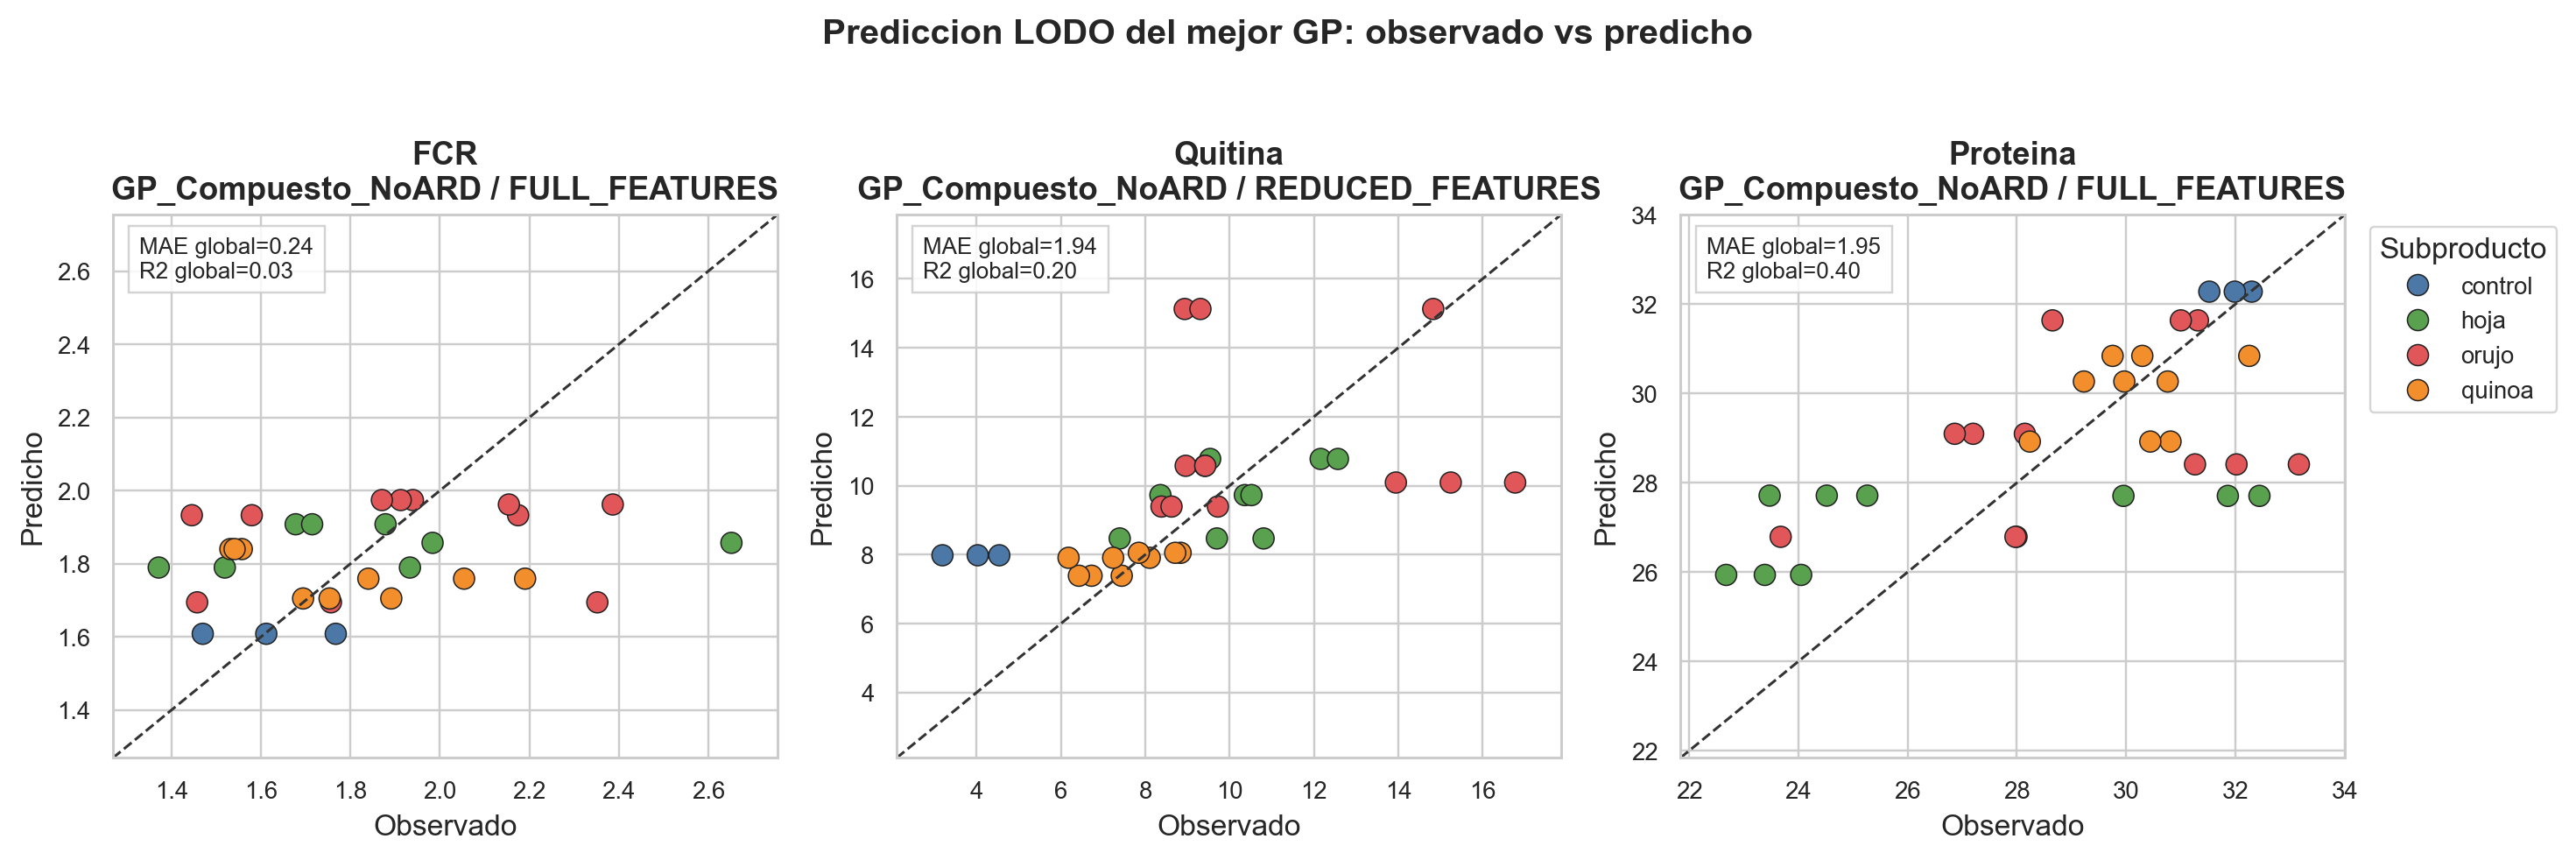
\includegraphics[width=\textwidth]{assets/app_real_best_gp_parity_by_target.png}
\caption[Paridad LODO del mejor GP]{Predicciones LODO del mejor GP por objetivo frente a los valores observados. Cada punto corresponde a una réplica experimental y el color indica el tipo de subproducto.}
\label{fig:app_real_best_gp_parity_by_target}
\end{figure}
\FloatBarrier

Esta figura permite detectar patrones que quedan ocultos en el MAE macro. En FCR, las predicciones tienden a concentrarse en un intervalo estrecho, lo que indica dificultad para extrapolar entre dietas. En quitina y proteína se observa una señal más clara, aunque con errores relevantes en algunos subproductos. Por tanto, el modelo aporta información útil, pero no debe interpretarse como sustituto del ensayo experimental.

\section{Contrastes LODO frente al modelo base Dummy}
\label{app:contrastes_lodo_dummy}

Los resultados LODO del caso real también permiten una lectura estadística complementaria, aunque necesariamente prudente por el tamaño muestral. En este análisis, cada dieta retenida en validación LODO se utiliza como unidad emparejada, de modo que los modelos se comparan sobre las mismas particiones de entrenamiento y prueba. La métrica utilizada es el MAE por dieta, ya que es la métrica principal del análisis de generalización.

Se aplicó primero un test de Friedman por objetivo para comparar todos los modelos disponibles. Después, como contraste dirigido frente al modelo base, se aplicó un test de rangos con signo de Wilcoxon unilateral entre el Dummy y el GP con mejor rango medio en cada objetivo. Los \(p\)-valores deben interpretarse como evidencia exploratoria, no como una prueba concluyente, porque cada objetivo dispone solo de 11 dietas.

\begin{table}[htbp]
\centering
\scriptsize
\caption[Contrastes LODO frente a Dummy]{Contrastes complementarios sobre el MAE LODO por dieta frente al modelo base Dummy. \(\Delta\)MAE representa \(MAE_{\mathrm{Dummy}}-MAE_{\mathrm{GP}}\), por lo que valores positivos favorecen al GP.}
\label{tab:app_lodo_dummy_contrasts}
\renewcommand{\arraystretch}{1.15}
\begin{tabularx}{\textwidth}{@{}p{1.4cm} p{2.7cm} r r r r X@{}}
\toprule
\textbf{Objetivo} & \textbf{GP de referencia} & \textbf{Rango} & \textbf{\(p_F\)} & \textbf{Mejora} & \textbf{\(\Delta\)MAE med.} & \textbf{Lectura} \\
\midrule
FCR & GP\_Matern32\_NoARD & 3.455 & 0.521 & 8/11 & 0.017 & Tendencia favorable al GP, pero sin evidencia concluyente frente al Dummy \((p=0.062)\). \\
Proteína & GP\_Matern32\_ARD & 3.273 & 0.209 & 9/11 & 0.827 & Evidencia favorable al GP frente al Dummy \((p=0.034)\); otros kernels GP también muestran mejoras significativas exploratorias. \\
Quitina & GP\_Linear & 2.636 & 0.194 & 8/11 & 0.380 & Mejora mediana positiva, pero contraste no concluyente \((p=0.160)\). \\
\bottomrule
\end{tabularx}
\end{table}
\FloatBarrier

La lectura principal de estos contrastes es coherente con las figuras de paridad y con las métricas agregadas. En proteína, el modelo GP aporta una mejora más consistente respecto al modelo base. En FCR se observa una señal débil, compatible con la dificultad de extrapolar entre dietas y con la concentración de las predicciones en un rango estrecho. En quitina, aunque algunos folds favorecen al GP, la evidencia no es suficiente para afirmar una mejora estadísticamente robusta con los datos disponibles.

\section{Intervalos predictivos por dieta}
\label{app:intervalos_prediccion_dieta}

La Figura~\ref{fig:app_prediction_intervals_by_diet} muestra, para cada dieta retenida en validación LODO, la media predictiva del GP junto con intervalos aproximados del \(95\,\%\). Esta visualización complementa el análisis de calibración presentado en la Sección~\ref{subsubsec:calibracion_incertidumbre_caso_real}, ya que permite observar de forma desagregada en qué dietas los intervalos contienen razonablemente los valores observados y en cuáles aparecen fallos concretos de cobertura.

\begin{figure}[htbp]
    \centering
    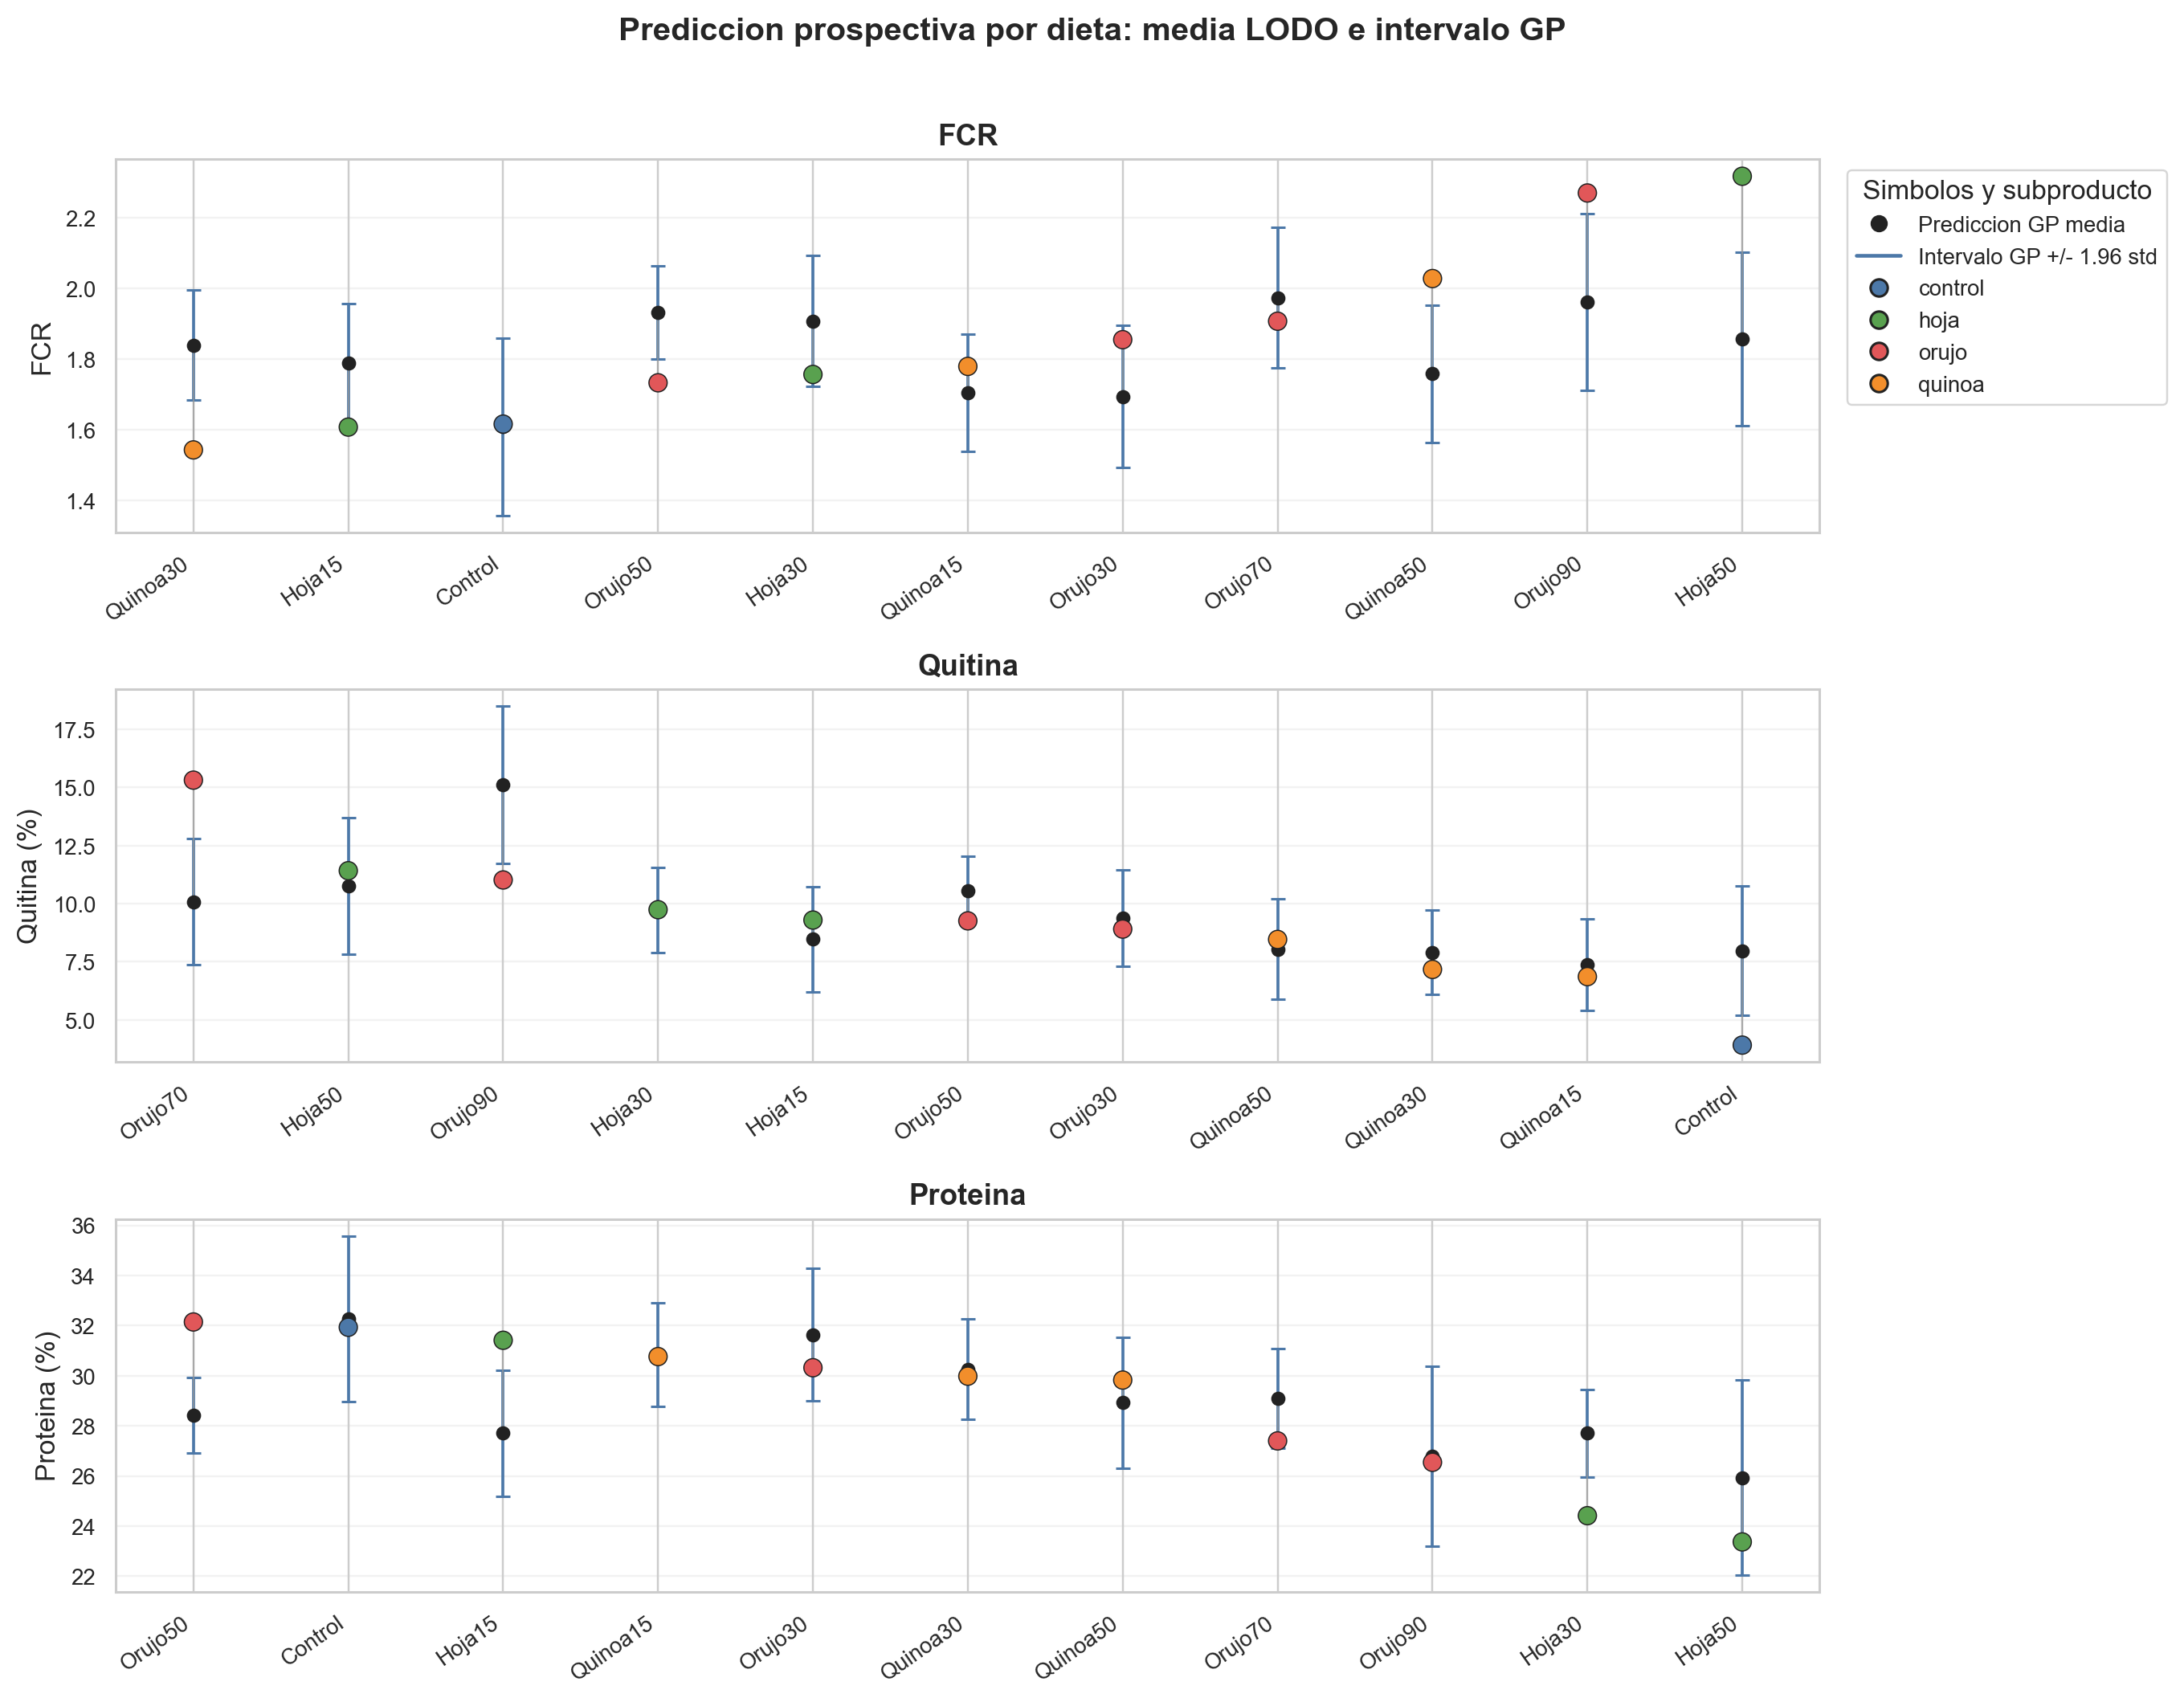
\includegraphics[width=0.95\textwidth]{assets/fig_06_prediction_intervals_by_diet.png}
    \caption[Intervalos predictivos por dieta]{Intervalos predictivos por dieta bajo validación LODO. Los puntos negros representan la media predictiva del GP y las barras muestran intervalos aproximados del \(95\,\%\) construidos como \(\mu \pm 1.96\sigma\). Los puntos coloreados corresponden a los valores observados por tipo de subproducto.}
    \label{fig:app_prediction_intervals_by_diet}
\end{figure}
\FloatBarrier

\section{Paisaje prospectivo de EI}
\label{app:ei_landscape_caso_real}

La Figura~\ref{fig:app_ei_candidate_landscape} muestra el paisaje prospectivo de EI sobre la rejilla factible de formulaciones considerada en el caso real. Esta visualización complementa el cribado presentado en la Sección~\ref{subsubsec:preinfill_caso_real}, donde se comparan los incumbents observados con los candidatos no ensayados priorizados por EI.

El objetivo de esta figura no es demostrar que los candidatos propuestos sean óptimos, sino mostrar cómo el criterio de adquisición distribuye el valor prospectivo sobre el espacio de búsqueda. Las zonas con mayor EI corresponden a combinaciones en las que el modelo identifica una posible mejora respecto al estado observado o una incertidumbre suficientemente relevante como para justificar una evaluación futura.

\begin{figure}[htbp]
    \centering
    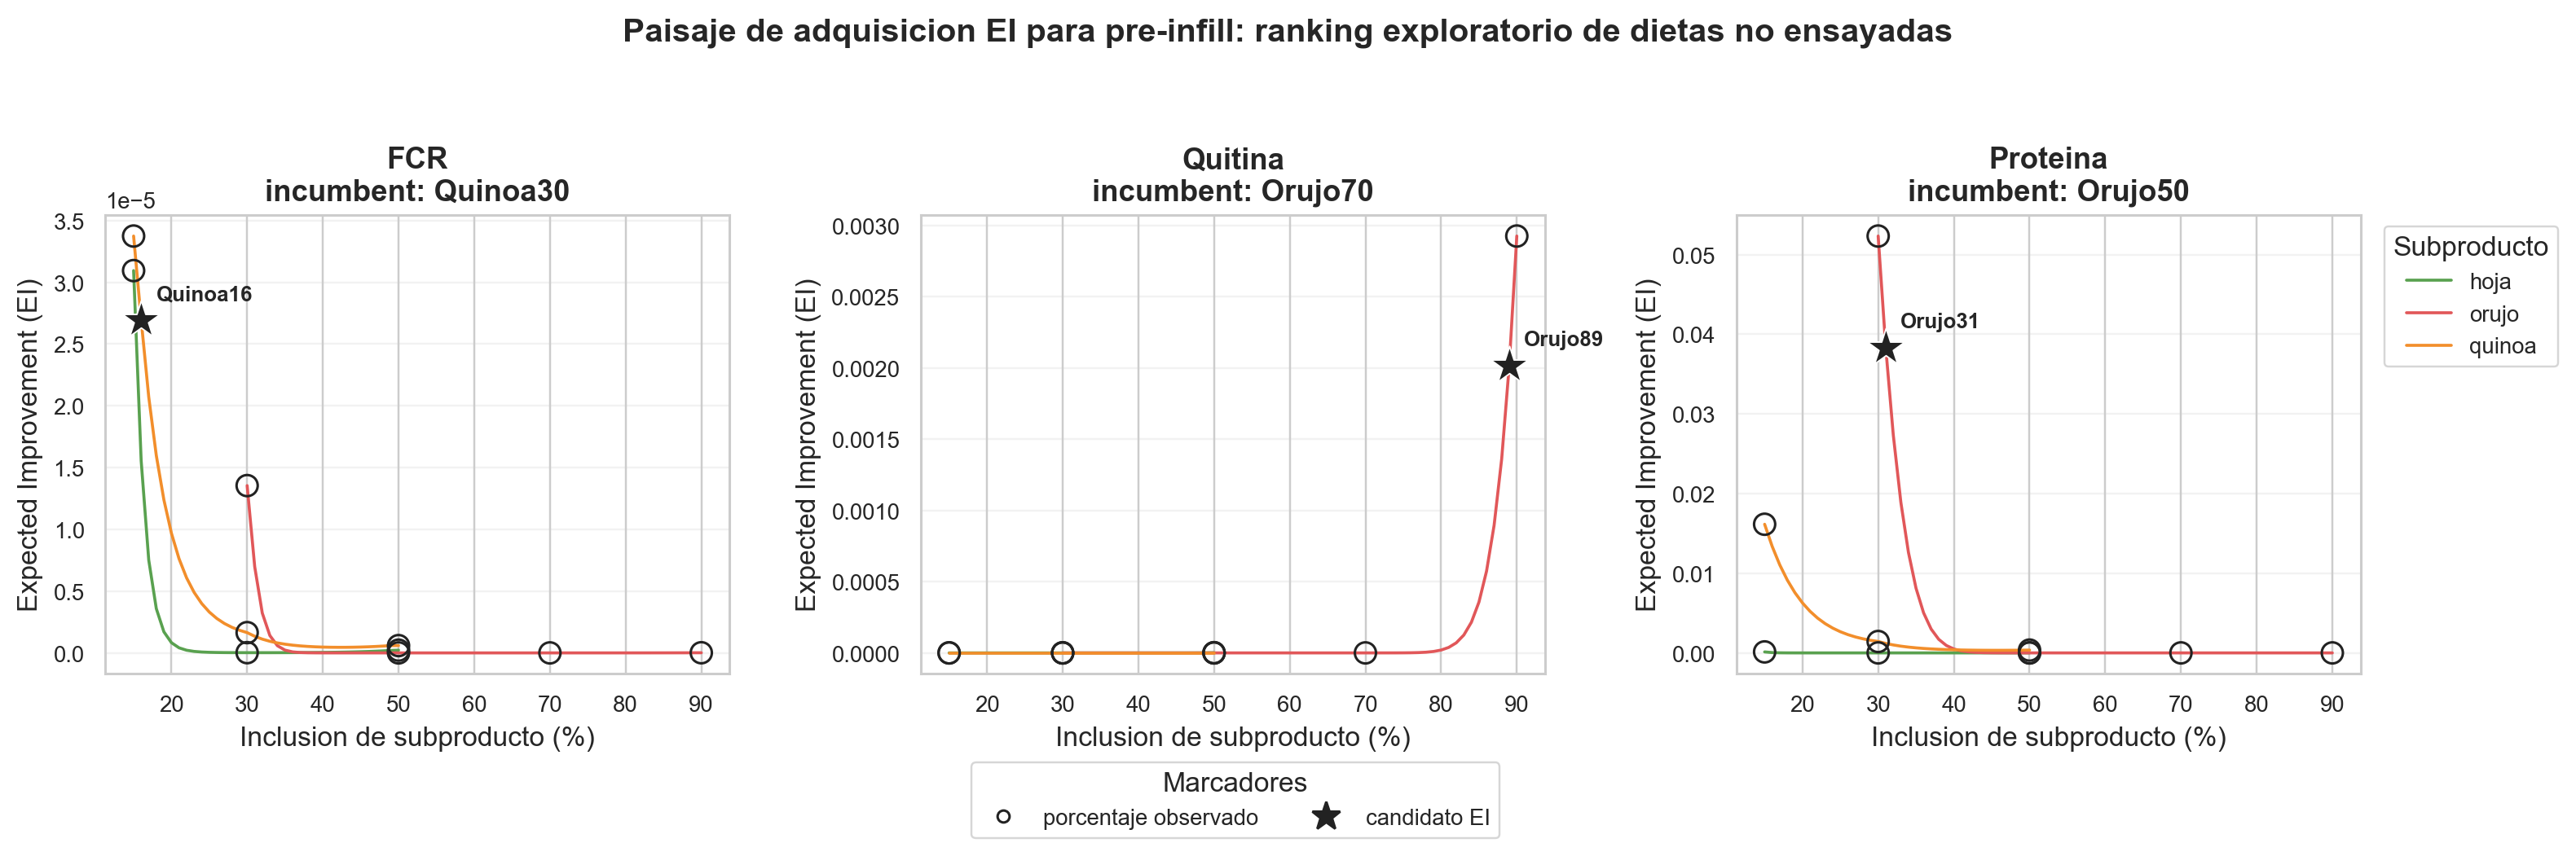
\includegraphics[width=0.95\textwidth]{assets/fig_08_ei_candidate_landscape.png}
    \caption[Paisaje prospectivo de EI]{Paisaje prospectivo de EI sobre la rejilla factible de formulaciones. Los máximos de EI identifican puntos candidatos para una posible evaluación futura, combinando predicción media e incertidumbre del GP.}
    \label{fig:app_ei_candidate_landscape}
\end{figure}

Por tanto, esta figura debe interpretarse como una herramienta de apoyo al diseño experimental posterior. En el estado actual del trabajo, los puntos destacados por EI constituyen hipótesis de ensayo y no resultados experimentales validados.
